\section{이론적 배경}

% --------------------------------------------------------------------
% 이 파일의 역할
% --------------------------------------------------------------------
% 2-Theorical_background.tex에는 연구 주제를 이해하는 데 필요한 이론적 배경을 씁니다.
% 핵심 개념의 정의, 관련 이론, 선행 연구의 흐름, 본 연구의 분석 관점을 정리합니다.
% 서론이 연구의 필요성을 제시하는 장이라면, 이론적 배경은 연구 문제를 해석할
% 개념적 틀과 학문적 근거를 세우는 장입니다.
%
% --------------------------------------------------------------------
% 이론적 배경 장 작성 안내
% --------------------------------------------------------------------
% 이 장에서는 연구 주제를 이해하는 데 필요한 개념, 이론, 선행 연구의 흐름을
% 체계적으로 정리합니다. 서론이 "왜 이 연구가 필요한가"를 설명한다면,
% 이론적 배경은 "이 연구가 어떤 학문적 논의 위에 서 있는가"를 보여 줍니다.
%
% 작성 순서 예시
% 1. 핵심 개념 정의
% 2. 관련 이론 또는 모형
% 3. 국내외 선행 연구
% 4. 선행 연구의 한계와 본 연구의 분석 관점
%
% 주의할 점
% - 선행 연구를 단순 요약 목록으로 만들지 않습니다.
% - 연구 목적과 직접 관련된 개념과 문헌을 중심으로 정리합니다.
% - 각 절의 끝에서는 본 연구와의 연결점을 짧게 정리합니다.

이론적 배경 장은 연구 주제를 이해하는 데 필요한 개념, 이론, 선행 연구를 정리하는 곳이다.
문헌을 한 편씩 나열하기보다 연구 흐름, 쟁점, 한계, 본 연구와의 연결점을 중심으로 묶어 서술한다.
각 절의 끝에서는 앞에서 검토한 내용이 본 연구의 연구 문제나 분석 관점과 어떻게 이어지는지 분명히 밝혀야 한다.

이 템플릿에서는 이론적 배경을 \verb|sub/2-Theorical_background.tex|에 작성한다.
문헌 정보는 \verb|sub/references.bib|에 저장하고, 본문에서는 한국어 문헌은 \verb|\ktextcite{}|와 \verb|\kparencite{}|로, 영어 문헌은 \verb|\textcite{}|와 \verb|\parencite{}|로 인용한다.
본문에서 실제로 인용한 문헌만 참고문헌 목록에 출력된다.

\subsection{핵심 개념}

% 연구에서 반복적으로 사용하는 핵심 개념을 정의합니다.
% 개념 정의는 사전식 정의보다 연구 맥락에서의 의미를 중심으로 씁니다.
% 여러 학자가 서로 다르게 정의한 개념이라면 공통점과 차이점을 정리한 뒤,
% 본 연구에서 사용할 조작적 정의를 제시합니다.

본 절에서는 연구 주제를 이해하는 데 필요한 핵심 개념을 정리한다.
개념을 정의할 때는 관련 문헌을 인용하고, 본 연구에서 해당 개념을 어떤 의미로 사용할 것인지 명확히 밝힌다.

\subsection{관련 이론}

% 연구 주제와 관련된 이론, 모형, 분석틀을 설명합니다.
% 이론을 소개할 때는 이론의 배경, 주요 구성 요소, 본 연구에 필요한 이유를 함께 씁니다.
% 그림이나 표를 활용하면 이론의 구조를 더 명확하게 보여 줄 수 있습니다.

관련 이론은 연구 문제를 해석하는 틀을 제공한다.
따라서 이 절에서는 본 연구가 어떤 이론적 관점에서 연구 대상을 바라보는지 설명한다.

\subsection{선행 연구}

% 선행 연구는 국내 연구와 국외 연구, 양적 연구와 질적 연구, 주제별 흐름 등
% 논문 주제에 맞는 기준으로 묶어서 서술합니다.
% 한 문단에 한 편씩 나열하기보다 쟁점별로 묶어 비교하는 것이 좋습니다.
%
% 인용 예시
% - 한국어 문헌: \ktextcite{kor_seo2009science}, (\kparencite{kor_seo2009science})
% - 영어 문헌: \textcite{eng_perkel2018jupyter}, (\parencite{eng_perkel2018jupyter})

선행 연구를 검토할 때는 연구 결과의 공통된 흐름과 차이를 함께 제시한다.
또한 기존 연구가 충분히 다루지 못한 부분을 정리하여 본 연구의 필요성과 연결한다.
생성형 AI가 추천한 논문을 활용할 때는 제목 검색, 저자와 연도 대조, DOI 확인, 원문 확인을 거친 뒤 실제 존재하는 문헌만 인용한다.
존재 여부가 확인되지 않거나 서지 정보가 서로 맞지 않는 문헌은 선행 연구 검토에서 제외한다.

\subsection{선행 연구 검토와 참고문헌 인용}

% 선행 연구 검토에서는 관련 연구를 단순히 하나씩 요약하는 데 그치지 않고,
% 연구 흐름과 쟁점을 중심으로 묶어서 서술합니다.
% 한국어 문헌은 \ktextcite, \kparencite를 사용하고,
% 영어 문헌은 \textcite, \parencite를 사용합니다.

선행 연구 검토를 작성할 때는 연구 주제와 직접 관련된 문헌을 중심으로 정리한다.
인용 표기 방법과 참고문헌 표기 방법은 학교, 학과, 학술지, 전공 분야에 따라 다를 수 있다.
따라서 최종 제출 전에는 반드시 소속 학교와 학과의 최신 학위논문 작성 지침을 확인해야 한다.
이 템플릿의 인용 및 참고문헌 형식은 APA 7판을 기반으로 하되, 한국어 문헌의 저자명 표기와 조사 처리 등 한글 문헌에 필요한 규칙을 추가한 것이다.
문헌을 인용할 때는 문장 속에서 저자를 언급하는 서술형 인용과 문장 끝에 근거를 제시하는 괄호형 인용을 구분하여 사용한다.

\ktextcite{kor_seo2009science}는 한국어 문헌을 문장 안에서 저자명 중심으로 인용하는 예시이다.
영어 문헌을 함께 제시해야 할 때는 관련 논의가 여러 연구에서 확인된다는 식으로 쓸 수 있다(\kparencite{kor_seo2009science}; \parencite{eng_perkel2018jupyter}).
이처럼 본문에 실제 인용 명령을 넣어야 문서 끝의 참고문헌 목록에 해당 문헌이 자동으로 출력된다.

\subsubsection{저자 수에 따른 인용 예시}

% 아래 예시는 sub/references.bib에 들어 있는 인용 예시용 BibTeX 항목을 실제로 부르는 방법입니다.
% 한국어 문헌은 \ktextcite와 \kparencite를 사용하고, 영어 문헌은 \textcite와 \parencite를 사용합니다.
% 이 템플릿에서는 \kparencite와 \parencite가 괄호를 직접 출력하지 않으므로,
% 괄호형 인용을 만들 때는 아래 예시처럼 본문에서 ( )를 직접 넣습니다.
% 실제 논문을 작성할 때는 아래 예시 문장을 삭제하고, 자신의 연구 주제에 맞는 실제 문헌을 인용합니다.

참고문헌을 인용할 때는 먼저 \verb|references.bib|에 문헌 정보를 입력하고, 본문에서 해당 \verb|bibcode|를 불러온다.
문장 안에서 저자를 주어처럼 언급할 때는 서술형 인용을 사용하고, 문장 끝에서 근거 문헌만 제시할 때는 괄호형 인용을 사용한다.
한국어 문헌은 \verb|\ktextcite{}|와 \verb|\kparencite{}|를 사용하고, 영어 문헌은 \verb|\textcite{}|와 \verb|\parencite{}|를 사용한다.

\paragraph{APA 7판의 저자 수별 본문 인용 원칙}
이 절의 예시는 APA 7판 기준을 따른다.
직접인용과 간접인용 모두 저자 수에 따른 본문 인용 규칙은 같으며, 직접인용에서는 여기에 쪽수나 쪽수 범위를 함께 적는다는 점만 다르다.
저자가 1명인 문헌은 처음 인용할 때와 다시 인용할 때 모두 그 저자명을 표시한다.
저자가 2명인 문헌도 처음 인용과 재인용 모두 두 저자명을 함께 표시한다.
한국어 문헌은 두 저자 사이를 ``와/과''로 연결하고, 영어 문헌은 APA 7판의 영문 저자 연결 방식에 따라 표시한다.
저자가 3명 이상인 문헌은 APA 7판에서 처음 인용할 때부터 재인용할 때까지 첫 번째 저자만 쓰고 나머지 저자는 축약한다.
이 템플릿에서는 한국어 문헌은 ``홍길동 외'', 영어 문헌은 ``Hong et al.''처럼 표시된다.
다만 서로 다른 문헌이 같은 첫 저자, 같은 연도, 비슷한 저자 조합을 가져 축약형만으로 구분되지 않을 때는 모호성을 피하기 위해 필요한 만큼 저자명을 더 표시해야 한다.

\paragraph{직접인용과 간접인용}
간접인용은 원문의 핵심 의미를 연구자가 자신의 문장으로 바꾸어 서술하는 방식이다.
선행 연구의 결과, 주장, 개념을 논문의 흐름에 맞게 요약하거나 재구성할 때 주로 사용한다.
간접인용에서는 따옴표를 붙이지 않지만, 원문의 주장이나 아이디어를 가져온 것이므로 반드시 출처를 표시한다.
특정 쪽의 논의를 자세히 풀어 쓴 경우에는 직접인용이 아니더라도 쪽수를 함께 적을 수 있다.

직접인용은 원문의 표현을 따옴표 안에 그대로 옮기는 방식이다.
원문 표현 자체가 중요하거나, 특정 개념 정의를 정확히 제시해야 할 때 제한적으로 사용한다.
직접인용을 할 때는 따옴표를 사용하고, 가능하면 쪽수를 함께 적어 원문 위치를 확인할 수 있게 한다.
긴 직접인용은 본문 흐름을 끊을 수 있으므로 꼭 필요한 경우에만 사용하고, 가능한 한 자신의 말로 요약하는 간접인용을 기본으로 삼는 것이 좋다.
직접인용과 간접인용 모두 원문 출처를 정확히 밝혀야 한다.
원문의 문장, 아이디어, 자료, 표, 그림을 가져오면서 출처를 표시하지 않거나 부정확하게 표시하면 표절로 판단될 수 있으므로, 본문 인용과 참고문헌 목록을 함께 확인한다.

\paragraph{간접인용 예시}
아래 예시는 저자 수와 문헌 언어에 따라 간접인용이 어떻게 표시되는지 보여 준다.
서술형 인용은 문장 안에서 저자를 드러내고, 괄호형 인용은 문장 끝에서 근거 문헌을 제시한다.

\begin{itemize}
    \item 저자 1명 한국어 논문: \ktextcite{kor_cite_example_one_author}는 과학 탐구 활동이 학습자의 개념 이해를 돕는다고 보았다. 괄호형으로는 과학 탐구 활동이 학습자의 개념 이해를 돕는다고 볼 수 있다(\kparencite{kor_cite_example_one_author}).
    \item 저자 1명 영어 논문: \textcite{eng_cite_example_one_author}는 과학 탐구 활동이 학습자의 개념 이해를 돕는다고 보았다. 괄호형으로는 과학 탐구 활동이 학습자의 개념 이해를 돕는다고 볼 수 있다(\parencite{eng_cite_example_one_author}).
    \item 저자 2명 한국어 논문: \ktextcite{kor_cite_example_two_authors}는 학생 질문이 탐구 과정의 중요한 단서라고 보았다. 괄호형으로는 학생 질문이 탐구 과정의 중요한 단서라고 볼 수 있다(\kparencite{kor_cite_example_two_authors}).
    \item 저자 2명 영어 논문: \textcite{eng_cite_example_two_authors}는 학생 질문이 탐구 과정의 중요한 단서라고 보았다. 괄호형으로는 학생 질문이 탐구 과정의 중요한 단서라고 볼 수 있다(\parencite{eng_cite_example_two_authors}).
    \item 저자 3명 한국어 논문: \ktextcite{kor_cite_example_three_authors}는 학습자의 질문 생성이 개념 이해와 관련된다고 보았다. 괄호형으로는 학습자의 질문 생성이 개념 이해와 관련된다고 볼 수 있다(\kparencite{kor_cite_example_three_authors}).
    \item 저자 3명 영어 논문: \textcite{eng_cite_example_three_authors}는 학습자의 질문 생성이 개념 이해와 관련된다고 보았다. 괄호형으로는 학습자의 질문 생성이 개념 이해와 관련된다고 볼 수 있다(\parencite{eng_cite_example_three_authors}).
    \item 저자 6명 한국어 논문: \ktextcite{kor_cite_example_six_authors}는 협력적 탐구 활동이 과학적 설명 구성을 촉진한다고 보았다. 괄호형으로는 협력적 탐구 활동이 과학적 설명 구성을 촉진한다고 볼 수 있다(\kparencite{kor_cite_example_six_authors}).
    \item 저자 6명 영어 논문: \textcite{eng_cite_example_six_authors}는 협력적 탐구 활동이 과학적 설명 구성을 촉진한다고 보았다. 괄호형으로는 협력적 탐구 활동이 과학적 설명 구성을 촉진한다고 볼 수 있다(\parencite{eng_cite_example_six_authors}).
    \item 저자 8명 한국어 논문: \ktextcite{kor_cite_example_eight_authors}는 수업 담화가 탐구 참여 양상과 연결된다고 보았다. 괄호형으로는 수업 담화가 탐구 참여 양상과 연결된다고 볼 수 있다(\kparencite{kor_cite_example_eight_authors}).
    \item 저자 8명 영어 논문: \textcite{eng_cite_example_eight_authors}는 수업 담화가 탐구 참여 양상과 연결된다고 보았다. 괄호형으로는 수업 담화가 탐구 참여 양상과 연결된다고 볼 수 있다(\parencite{eng_cite_example_eight_authors}).
\end{itemize}

여러 문헌의 논의를 함께 요약할 때는 ``관련 논의는 여러 연구에서 확인된다(\kparencite{kor_cite_example_two_authors}; \parencite{eng_cite_example_two_authors})''처럼 세미콜론으로 문헌을 구분하여 제시할 수 있다.

\paragraph{직접인용 예시}
짧은 직접인용은 원문의 문장을 따옴표 안에 넣고, 인용 뒤에 저자, 연도, 쪽수를 함께 제시한다.
아래 예시는 저자 수와 문헌 언어에 따라 직접인용 출처가 어떻게 표시되는지 보여 준다.
영어 논문을 직접 인용할 때는 원문 표현을 영어 그대로 옮기고 쪽수를 함께 적는다.

\begin{itemize}
    \item 저자 1명 한국어 논문: ``학습자의 질문은 탐구의 출발점이다''(\kparencite{kor_cite_example_one_author}, p.~3).
    \item 저자 1명 영어 논문: ``questions can guide inquiry''(\parencite{eng_cite_example_one_author}, p.~3).
    \item 저자 2명 한국어 논문: ``학생 질문은 탐구 과정의 중요한 단서이다''(\kparencite{kor_cite_example_two_authors}, p.~15).
    \item 저자 2명 영어 논문: ``student questions support inquiry''(\parencite{eng_cite_example_two_authors}, p.~15).
    \item 저자 3명 한국어 논문: ``질문 생성은 개념 이해와 관련된다''(\kparencite{kor_cite_example_three_authors}, p.~24).
    \item 저자 3명 영어 논문: ``question generation supports understanding''(\parencite{eng_cite_example_three_authors}, p.~24).
    \item 저자 6명 한국어 논문: ``협력적 탐구는 설명 구성을 촉진한다''(\kparencite{kor_cite_example_six_authors}, p.~35).
    \item 저자 6명 영어 논문: ``collaborative inquiry supports the construction of explanations''(\parencite{eng_cite_example_six_authors}, p.~35).
    \item 저자 8명 한국어 논문: ``수업 담화는 탐구 참여 양상과 연결된다''(\kparencite{kor_cite_example_eight_authors}, p.~46).
    \item 저자 8명 영어 논문: ``classroom discourse is connected to patterns of inquiry participation''(\parencite{eng_cite_example_eight_authors}, p.~46).
\end{itemize}

인용문이 두세 문장 이상으로 길어지는 경우에는 본문 안에 이어 쓰기보다 별도 문단으로 제시할 수 있다.
다만 긴 직접인용은 논문의 논리 흐름을 약하게 만들 수 있으므로, 원문 표현 자체가 분석 대상이거나 정의를 정확히 제시해야 하는 경우에만 사용한다.

\begin{quote}
    과학 수업에서 탐구는 학생이 이미 정해진 절차를 따라가는 활동에 머물지 않는다.
    학생은 관찰, 질문, 증거 해석의 과정을 거치며 과학 개념을 자신의 언어로 재구성한다(\kparencite{kor_cite_example_two_authors}, pp.~23--24).
\end{quote}

긴 문단을 직접인용할 때는 인용문 앞뒤로 본문과 구분되는 여백을 두고, 인용문 전체를 별도 블록으로 제시한다.
이때 본문 속 짧은 직접인용처럼 따옴표를 붙이기보다, 들여쓰기된 인용 블록 자체로 직접인용임을 드러내는 방식이 일반적이다.
인용문 뒤에는 출처와 쪽수 범위를 적고, 인용문 다음 문단에서는 그 인용문이 본 연구의 논의와 어떻게 연결되는지 해석한다.

\begin{quote}
    과학 수업에서 학생의 질문은 단순히 교사의 설명을 확인하는 절차가 아니라, 학습자가 현상을 어떻게 이해하고 있는지를 드러내는 중요한 단서이다.
    특히 탐구 활동에서 학생이 제기하는 질문은 관찰한 현상, 기존 지식, 동료와의 상호작용이 만나는 지점에서 형성된다.
    따라서 교사는 질문의 정답 여부만 판단하기보다, 그 질문이 어떤 개념적 어려움과 탐구 가능성을 포함하고 있는지 해석할 필요가 있다(\kparencite{kor_cite_example_three_authors}, pp.~31--32).
\end{quote}

위와 같이 긴 문단을 인용한 뒤에는 ``위 인용문은 과학 수업에서 학생 질문을 탐구의 출발점으로 해석해야 함을 보여 준다''와 같이 연구자의 해석을 이어서 제시한다.
직접인용만 제시하고 설명을 덧붙이지 않으면 독자가 그 인용문이 연구 문제와 어떤 관련이 있는지 판단하기 어렵다.

위 예시는 직접인용의 형식을 보여 주기 위한 예시 문장이다.
실제 논문에서는 반드시 원문과 정확히 일치하는 문장을 사용하고, 해당 문장이 실린 정확한 쪽수를 확인해야 한다.

\paragraph{Google Scholar에서 BibTeX 가져오기}
Google Scholar에서 논문 제목을 검색한 뒤, 검색 결과 아래에 있는 따옴표 모양의 인용 아이콘을 누르면 그림 \ref{fig:google-scholar-bibtex}과 같은 인용 창이 나타난다.
인용 창 아래쪽에는 여러 내보내기 형식이 표시되며, 그중 \verb|BibTeX|를 선택한다.

\begin{figure}[htbp]
    \centering
    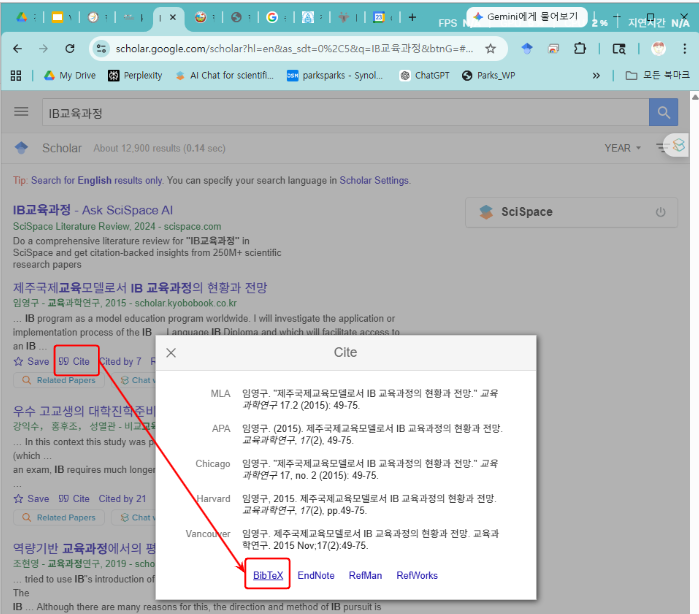
\includegraphics[width=0.85\linewidth]{images/bibtex.png}
    \caption{Google Scholar 인용 창에서 BibTeX를 선택하는 예}
    \label{fig:google-scholar-bibtex}
\end{figure}

\verb|BibTeX|를 선택하면 새 화면에 \verb|@article|, \verb|@book| 등으로 시작하는 BibTeX 항목이 출력된다.
이 항목 전체를 복사하여 \path{sub/references.bib} 파일에 붙여 넣는다.

Google Scholar에서 가져온 BibTeX는 자동 생성 정보이므로 저자명, 논문 제목, 학술지명, 출판 연도, 권호, 페이지, DOI를 PDF 첫 페이지나 학술지 공식 페이지와 대조한 뒤 사용한다.
영어로 작성하는 논문에서는 일반적인 APA 7판 BibTeX 형식을 그대로 활용해도 되는 경우가 많지만, 이 템플릿처럼 한글 논문을 작성하면서 한국어 문헌과 영어 문헌을 함께 인용할 때는 아래와 같이 항목을 정리하는 것이 좋다.

먼저 인용 키를 이 템플릿의 규칙에 맞게 한국어 문헌과 영어 문헌이 구분되도록 바꾼다.
예를 들어 한국어 논문은 \verb|kor_hong2026|처럼, 영어 논문은 \verb|eng_hong2026|처럼 짧고 알아보기 쉽게 정할 수 있다.
또한 Google Scholar가 만든 BibTeX에는 \verb|langid|가 없을 수 있다.
한국어 문헌에는 \verb|korean|, 영어 문헌에는 \verb|english| 값을 추가한다.

저자가 1명인 경우, 한국어 문헌은 \ktextcite{kor_cite_example_one_author}처럼 쓸 수 있고, 영어 문헌은 \textcite{eng_cite_example_one_author}처럼 쓸 수 있다.
괄호형 인용은 한국어 문헌의 경우 (\kparencite{kor_cite_example_one_author}), 영어 문헌의 경우 (\parencite{eng_cite_example_one_author})처럼 쓴다.
처음 인용할 때와 다시 인용할 때의 표기는 같다.

저자가 2명인 경우, 한국어 문헌은 \ktextcite{kor_cite_example_two_authors}처럼 두 저자 사이에 한국어 연결어가 들어가고, 영어 문헌은 \textcite{eng_cite_example_two_authors}처럼 영문 APA 형식에 맞게 표시된다.
괄호형 인용은 (\kparencite{kor_cite_example_two_authors}) 또는 (\parencite{eng_cite_example_two_authors})처럼 작성한다.
처음 인용할 때와 다시 인용할 때 모두 두 저자명을 표시한다.

저자가 3명 이상인 경우에는 APA 7판 기준에 따라 처음 인용할 때부터 본문 인용에서 첫 번째 저자 중심으로 축약하여 표시한다.
이때 한국어 문헌은 ``홍길동 외''처럼 표시하고, 영어 문헌은 ``Hong et al.''처럼 표시한다.
다시 인용할 때도 같은 축약형을 사용하므로, APA 6판처럼 첫 인용에서만 모든 저자를 쓰고 이후에 줄이는 방식과 다르다.
예를 들어 저자 3명 문헌은 \ktextcite{kor_cite_example_three_authors} 또는 \textcite{eng_cite_example_three_authors}처럼 인용하고, 괄호형으로는 (\kparencite{kor_cite_example_three_authors}) 또는 (\parencite{eng_cite_example_three_authors})처럼 쓴다.

저자가 6명인 문헌도 같은 방식으로 처리한다.
한국어 문헌은 \ktextcite{kor_cite_example_six_authors}와 같이 쓰고, 영어 문헌은 \textcite{eng_cite_example_six_authors}와 같이 쓴다.
괄호형 인용은 (\kparencite{kor_cite_example_six_authors}) 또는 (\parencite{eng_cite_example_six_authors})처럼 작성한다.

저자가 8명인 문헌도 본문에서는 같은 원칙을 따른다.
한국어 문헌은 \ktextcite{kor_cite_example_eight_authors}처럼, 영어 문헌은 \textcite{eng_cite_example_eight_authors}처럼 인용한다.
괄호형 인용은 (\kparencite{kor_cite_example_eight_authors}) 또는 (\parencite{eng_cite_example_eight_authors})처럼 쓴다.
저자 3명, 6명, 8명 문헌은 모두 처음 인용과 재인용의 축약 방식이 같다.

한국어 문헌과 영어 문헌을 한 괄호 안에 함께 제시할 때는 한국어 문헌을 먼저 쓰고 세미콜론 뒤에 영어 문헌을 쓴다.
예를 들어 저자 2명 문헌을 함께 인용하면 (\kparencite{kor_cite_example_two_authors}; \parencite{eng_cite_example_two_authors})처럼 작성할 수 있다.
이 예시는 실제 출력에서 ``홍길동과 임꺽정, 2026; Hong and Im, 2026''처럼 한국어 문헌이 앞에 오고 영어 문헌이 뒤에 오는 형태를 의도한 것이다.
한국어 논문과 영어 논문은 저자 연결어, 쉼표, 축약 표기 방식이 서로 다르므로 하나의 인용 명령으로 모두 처리하기 어렵다.
그래서 이 템플릿에서는 한국어 문헌에는 \verb|\kparencite{}|를, 영어 문헌에는 \verb|\parencite{}|를 적용해 두었다.
두 명령은 인용 내용만 출력하고 바깥 괄호는 직접 쓰도록 되어 있으므로, 한국어 문헌을 앞에 두고 영어 문헌을 뒤에 두는 혼합 인용 형식을 작성자가 자연스럽게 조절할 수 있다.

\subsubsection{생성형 AI가 제시한 선행 연구 확인 방법}

% 생성형 AI는 선행 연구 탐색의 출발점으로 활용할 수 있지만,
% 실제로 존재하지 않는 논문 제목, 잘못된 저자명, 틀린 연도, 존재하지 않는 DOI,
% 서로 다른 논문의 정보를 섞은 참고문헌을 제시할 수 있습니다.
% 따라서 AI가 알려 준 문헌은 바로 인용하지 말고, 반드시 연구자가 직접 확인해야 합니다.

생성형 AI가 제시한 선행 연구 목록은 참고문헌 후보로만 사용한다.
AI가 제시한 논문을 실제 논문으로 인용하기 전에는 다음 절차에 따라 존재 여부와 서지 정보를 확인한다.

\begin{enumerate}
    \item \textbf{제목을 그대로 검색한다.}
    논문 제목 전체를 따옴표로 묶어 Google Scholar, RISS, DBpia, KCI, Scopus, Web of Science, 학술지 누리집 등에서 검색한다.
    제목이 정확히 검색되지 않으면 제목 일부, 핵심어, 저자명을 조합하여 다시 검색한다.

    \item \textbf{저자, 연도, 학술지명을 대조한다.}
    검색 결과에서 논문 제목이 비슷하더라도 저자명, 출판 연도, 학술지명, 권호, 페이지가 AI가 제시한 정보와 일치하는지 확인한다.
    한두 항목이 다르면 단순 오탈자일 수 있지만, 여러 항목이 다르면 AI가 서로 다른 문헌 정보를 섞었을 가능성이 있다.

    \item \textbf{DOI 또는 공식 URL을 확인한다.}
    DOI가 제시된 경우 DOI 검색 사이트나 출판사 페이지에서 DOI가 실제 논문으로 연결되는지 확인한다.
    DOI가 다른 제목으로 연결되거나 검색되지 않으면 해당 DOI를 참고문헌에 사용하지 않는다.

    \item \textbf{원문 또는 초록을 직접 읽는다.}
    논문이 실제로 존재하더라도 연구 주제와 무관할 수 있다.
    따라서 초록, 연구 목적, 연구 방법, 주요 결과를 직접 확인하고, 본 연구의 선행 연구 검토에 포함할 필요가 있는지 판단한다.

    \item \textbf{참고문헌 관리 프로그램에 직접 등록한다.}
    Zotero, EndNote, Mendeley, BibTeX 등으로 논문 정보를 가져온 뒤 제목, 저자, 연도, 학술지명, DOI를 다시 확인한다.
    자동으로 가져온 정보에도 오류가 있을 수 있으므로 PDF 첫 페이지나 학술지 공식 페이지와 대조한다.

    \item \textbf{확인되지 않은 문헌은 인용하지 않는다.}
    검색해도 원문, 초록, 학술지 페이지, DOI, 도서관 소장 정보가 확인되지 않는 문헌은 실제 존재 여부가 불확실하므로 학위논문에 인용하지 않는다.
\end{enumerate}

생성형 AI가 선행 연구의 내용을 요약해 준 경우에도 요약문을 그대로 신뢰해서는 안 된다.
반드시 원문을 읽고 연구자가 직접 연구 목적, 연구 방법, 연구 결과, 한계를 정리해야 한다.
AI의 요약은 문헌을 빠르게 훑어보기 위한 보조 자료일 뿐이며, 최종적인 문헌 선택과 해석의 책임은 논문 작성자에게 있다.

\subsection{본 연구의 분석 관점}

% 이 절에서는 앞에서 검토한 개념, 이론, 선행 연구를 바탕으로
% 본 연구가 어떤 관점에서 자료를 수집하고 분석할 것인지 정리합니다.
% 연구 방법 장으로 넘어가기 전에 이론적 배경과 연구 설계를 연결하는 역할을 합니다.

본 연구는 앞서 검토한 개념과 선행 연구를 바탕으로 연구 문제를 구체화한다.
이 분석 관점은 다음 장의 연구 방법에서 자료 수집과 분석 절차를 설계하는 기준으로 사용된다.
